\documentclass[aspectratio=169,14pt]{beamer}
\usetheme{default}
\usepackage{fontspec}
\setmainfont{texgyrepagella-regular.otf}[BoldFont=texgyrepagella-bold.otf,ItalicFont=texgyrepagella-italic.otf,BoldItalicFont=texgyrepagella-bolditalic.otf]
\setsansfont{texgyreheros-regular.otf}[BoldFont=texgyreheros-bold.otf,ItalicFont=texgyreheros-italic.otf,BoldItalicFont=texgyreheros-bold.otf,BoldItalicFeatures={FakeSlant=0.2}]
\setmonofont{lmmono10-regular.otf}[Scale=0.85]
\setbeamertemplate{navigation symbols}{}
\usepackage{pgfpages}
\newif\ifpresenter
\ifdefined\PresenterVersion\presentertrue\else\presenterfalse\fi
\ifpresenter
  \setbeameroption{show notes on second screen=right}
  \setbeamertemplate{note page}[plain]
\fi
\usepackage{amsmath,amssymb,bm,booktabs,array,graphicx,xcolor}
\usepackage{tikz,pgfplots,adjustbox,listings,xurl}
\pgfplotsset{compat=1.18}
\usetikzlibrary{arrows.meta,positioning,calc,fit,shapes.geometric,decorations.pathreplacing,patterns}
% UIUC official brand colors, verified 2026-10-23.
% https://brand.illinois.edu/visual-identity/color
\definecolor{IlliniOrange}{HTML}{FF5F05}
\definecolor{IlliniBlue}{HTML}{13294B}
\definecolor{Storm}{HTML}{707372}
\definecolor{LightStorm}{HTML}{C6C7C6}
\definecolor{Industrial}{HTML}{1D58A7}
\definecolor{Patina}{HTML}{007E8E}
\tikzset{>=Stealth, every node/.style={font=\small,text=IlliniBlue}, box/.style={draw=IlliniBlue,rounded corners=2pt,align=center,inner sep=6pt,execute at begin node=\hyphenpenalty10000\relax}, orangebox/.style={box,draw=IlliniOrange,very thick}, edge/.style={->,thick,IlliniBlue}, accent/.style={->,very thick,IlliniOrange}}
\pgfplotsset{every axis/.append style={width=13.5cm,height=6.5cm,axis line style={IlliniBlue},tick label style={font=\small,text=IlliniBlue},label style={font=\small,text=IlliniBlue},legend style={font=\small,draw=none,fill=white},grid style={LightStorm},major grid style={LightStorm},axis lines=left,clip=false}, every axis plot/.append style={thick}}

\definecolor{slidepaper}{RGB}{234,220,201}
\setbeamercolor{background canvas}{bg=slidepaper}
\setbeamercolor{normal text}{fg=IlliniBlue}
\setbeamercolor{frametitle}{fg=IlliniBlue}
\setbeamercolor{title}{fg=IlliniBlue}
\setbeamercolor{item}{fg=IlliniOrange}
\setbeamerfont{frametitle}{size=\large,series=\bfseries}
\setbeamerfont{title}{size=\Large,series=\bfseries}
\setbeamertemplate{itemize item}{\color{IlliniOrange}$\bullet$}
\setbeamertemplate{itemize subitem}{\color{IlliniOrange}\footnotesize$\circ$}
\setbeamercolor{orangerule}{bg=IlliniOrange}
\setbeamertemplate{headline}{\begin{beamercolorbox}[wd=\paperwidth,ht=0.1cm,dp=0.1cm]{orangerule}\end{beamercolorbox}}
\setbeamertemplate{footline}{\begin{beamercolorbox}[wd=\paperwidth,ht=0.1cm,dp=0.1cm]{orangerule}\end{beamercolorbox}}
\setbeamersize{text margin left=0.65cm,text margin right=0.65cm}
\setlength{\leftmargini}{1.1em}
\newenvironment{slidebullets}{\begin{itemize}\setlength\itemsep{0.8em}}{\end{itemize}}
\pgfplotsset{every axis/.append style={legend style={fill=slidepaper}}}
\lstdefinelanguage{CoursePython}{keywords={from,import,for,in,if,else,def,return,assert,True,False,None},sensitive=true,morecomment=[l]{\#},morestring=[b]',morestring=[b]"}
\lstset{language=CoursePython,basicstyle=\ttfamily\small,keywordstyle=\color{IlliniBlue}\bfseries,commentstyle=\color{Storm},stringstyle=\color{IlliniBlue},showstringspaces=false,breaklines=true,columns=fullflexible,keepspaces=true,frame=none,aboveskip=0.7em,belowskip=0.7em}
\newcommand{\E}{\mathbb E}
\newcommand{\Var}{\operatorname{Var}}
\newcommand{\Cov}{\operatorname{Cov}}
\hypersetup{colorlinks=true,urlcolor=IlliniBlue,linkcolor=IlliniBlue}

\title{Marketing Analytics}
\subtitle{Regression and Marketing Interpretation}
\author{By Nathan Yang}
\date{Session 04}
\begin{document}
\begin{frame}
\titlepage
\end{frame}
\begin{frame}{Competitors and Store Sales}
\usebeamercolor[fg]{normal text}
\vfill
\begin{slidebullets}
\item Stores in markets with more competitors can have higher sales.
\item Demand attracts firms and also raises sales.
\item The managerial question concerns the effect of an additional competitor.
\end{slidebullets}
\vfill
\note{A positive cross-market association can combine the negative competitive effect with the selection of firms into high-demand markets. The mechanism determines which comparison is informative.

M3, Section 3.3, Marketing Analytics Lecture Notes. \url{../06_Lecture_Notes/modules/M03_Regression.md}}
\end{frame}
\begin{frame}{A Conditional Mean}
\usebeamercolor[fg]{normal text}
\noindent Relate store sales to observed marketing conditions.
\medskip
\[
Y_i=\beta_0+\beta_1 X_i+\beta_2 Z_i+u_i
\]
\medskip
\noindent The coefficient on $X_i$ describes its linear association holding included $Z_i$ fixed.
\note{The outcome and regressors require explicit units and timing. A conditional association becomes a causal parameter only under the assumptions supplied by the design and model.

M3, Section 3.1, Marketing Analytics Lecture Notes. \url{../06_Lecture_Notes/modules/M03_Regression.md}}
\end{frame}
\begin{frame}{Ordinary Least Squares}
\usebeamercolor[fg]{normal text}
\vfill
\begin{slidebullets}
\item OLS chooses coefficients to minimize squared residuals.
\item A residual is observed sales minus fitted sales.
\item The model summarizes the comparison supplied by the data.
\end{slidebullets}
\vfill
\note{The fitted residuals sum to zero when an intercept is included and the usual OLS solution exists. This algebraic property does not establish independence between treatment and unobserved demand.

M3, Section 3.1, Marketing Analytics Lecture Notes. \url{../06_Lecture_Notes/modules/M03_Regression.md}}
\end{frame}
\begin{frame}{Omitted Demand Reverses the Sign}
\usebeamercolor[fg]{normal text}
\centering
\begingroup
\begin{adjustbox}{max width=0.98\textwidth,max totalheight=0.65\textheight}
% Original synthetic teaching figure; see corresponding module.
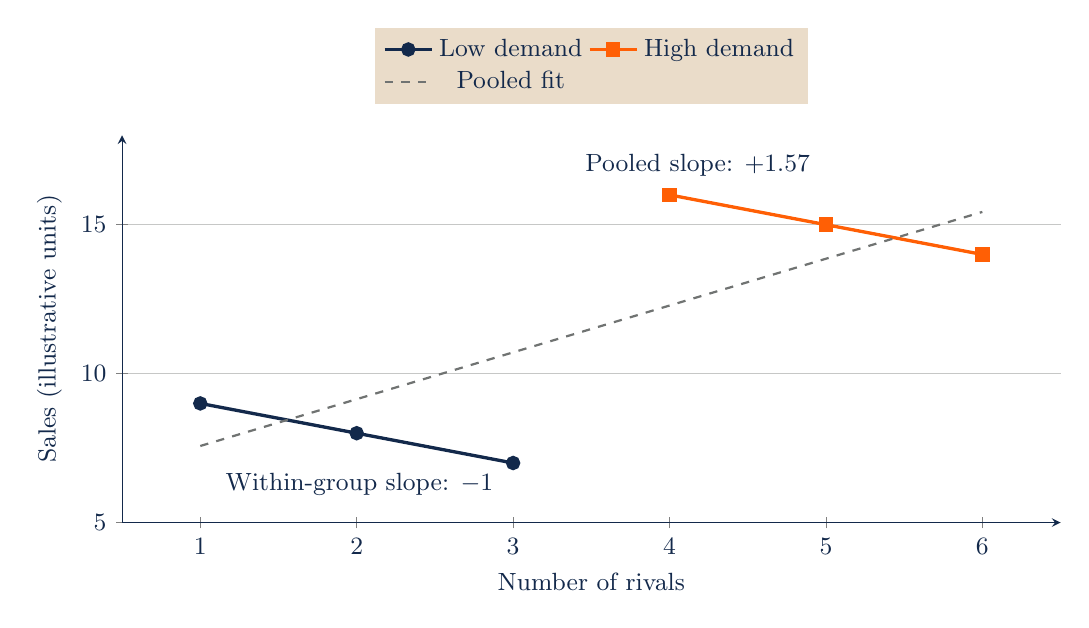
\begin{tikzpicture}
\begin{axis}[xmin=.5,xmax=6.5,ymin=5,ymax=18,xlabel={Number of rivals},ylabel={Sales (illustrative units)},legend style={at={(.5,1.08)},anchor=south,legend columns=2},xtick={1,...,6},ymajorgrids=true]
\addplot[IlliniBlue,mark=*,very thick] coordinates {(1,9)(2,8)(3,7)};
\addplot[IlliniOrange,mark=square*,very thick] coordinates {(4,16)(5,15)(6,14)};
\addplot[Storm,dashed,domain=1:6] {6+11*x/7};
\legend{Low demand,High demand,Pooled fit}
\node[anchor=west,font=\small] at (axis cs:1.1,6.3) {Within-group slope: $-1$};
\node[anchor=west,font=\small] at (axis cs:3.4,17) {Pooled slope: $+1.57$};
\end{axis}
\end{tikzpicture}

\end{adjustbox}
\endgroup
\par\medskip
{\small Synthetic markets hold the underlying competitive mechanism fixed.\par}
\note{Market demand affects both entry and sales. Controlling for a valid measure of demand can change the regression coefficient by changing which observations are compared.

M3, Section 3.3, Marketing Analytics Lecture Notes. \url{../06_Lecture_Notes/modules/M03_Regression.md}}
\end{frame}
\begin{frame}{Omitted-Variable Bias}
\usebeamercolor[fg]{normal text}
\noindent Suppose demand $Z$ affects sales and is omitted from a regression on $X$.
\medskip
\[
\widetilde\beta_1=\beta_1+\beta_2\frac{\Cov(X,Z)}{\Var(X)}
\]
\medskip
\noindent The omitted association can offset or reverse the coefficient of interest.
\note{This expression is the population linear-projection result under the stated model and orthogonality conditions. Its sign depends on both the effect of Z and its association with X.

M3, Section 3.2, Marketing Analytics Lecture Notes. \url{../06_Lecture_Notes/modules/M03_Regression.md}}
\end{frame}
\begin{frame}{Price and Sales Units}
\usebeamercolor[fg]{normal text}
\vfill
\begin{slidebullets}
\item A level coefficient is sales units per dollar.
\item A log-log price coefficient is an elasticity under the model.
\item The exact change for a log outcome uses an exponential transformation.
\end{slidebullets}
\vfill
\note{A coefficient on a binary regressor in a log-outcome model implies a multiplicative change of exp(beta)-1 under the relevant conditional interpretation. A percentage-point change in a probability is a different unit.

M3, Section 3.4, Marketing Analytics Lecture Notes. \url{../06_Lecture_Notes/modules/M03_Regression.md}}
\end{frame}
\begin{frame}{Interactions}
\usebeamercolor[fg]{normal text}
\noindent Allow a message association to vary with account tenure $T$.
\medskip
\[
Y=\beta_0+\beta_1 M+\beta_2 T+\beta_3 MT+u
\]
\medskip
\noindent The message comparison at tenure $T$ is $\beta_1+\beta_3T$.
\note{The main message coefficient applies at tenure zero under this parameterization. Centering tenure changes that reference point while leaving fitted values unchanged.

M3, Section 3.5, Marketing Analytics Lecture Notes. \url{../06_Lecture_Notes/modules/M03_Regression.md}}
\end{frame}
\begin{frame}{A Comparison Changes With Tenure}
\usebeamercolor[fg]{normal text}
\centering
\begingroup
\begin{adjustbox}{max width=0.98\textwidth,max totalheight=0.65\textheight}
% Original synthetic teaching figure; see corresponding module.
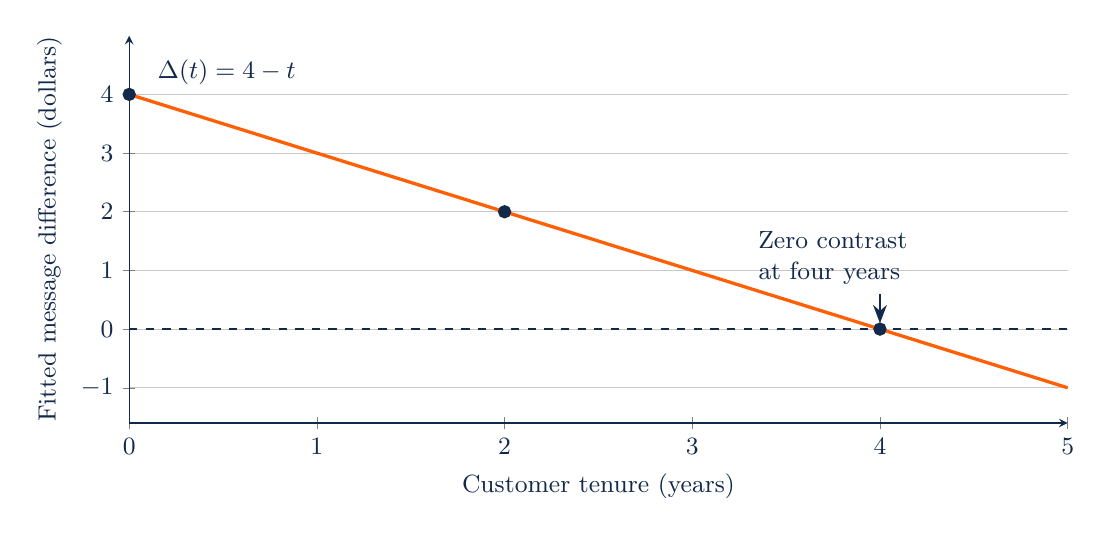
\begin{tikzpicture}
\begin{axis}[xmin=0,xmax=5,ymin=-1.6,ymax=5,xlabel={Customer tenure (years)},ylabel={Fitted message difference (dollars)},xtick={0,...,5},ytick={-1,0,1,2,3,4},ymajorgrids=true]
\addplot[IlliniOrange,very thick,domain=0:5] {4-x};
\addplot[IlliniBlue,dashed] coordinates {(0,0)(5,0)};
\addplot[IlliniBlue,only marks,mark=*] coordinates {(0,4)(2,2)(4,0)};
\node[anchor=south west] at (axis cs:.1,4) {$\Delta(t)=4-t$};
\node[anchor=south west,align=left] at (axis cs:3.3,.6) {Zero contrast\\at four years};
\draw[edge] (axis cs:4,.6)--(axis cs:4,.1);
\end{axis}
\end{tikzpicture}

\end{adjustbox}
\endgroup
\par\medskip
{\small Synthetic message-response model. Tenure determines the conditional comparison.\par}
\note{The marginal comparison should be reported at meaningful tenures within the observed support. A crossing outside the sample range is an extrapolation.

M3, Section 3.5, Marketing Analytics Lecture Notes. \url{../06_Lecture_Notes/modules/M03_Regression.md}}
\end{frame}
\begin{frame}{Uncertainty and Practical Importance}
\usebeamercolor[fg]{normal text}
\vfill
\begin{slidebullets}
\item Report effect size in managerial units.
\item Cluster at the unit that shares outcome disturbances or assignment.
\item Compare the interval with a decision-relevant magnitude.
\end{slidebullets}
\vfill
\note{A small p-value does not measure the size of an effect. A wide interval containing zero can also contain large economically consequential effects. The appropriate sampling unit depends on the design.

M3, Section 3.6, Marketing Analytics Lecture Notes. \url{../06_Lecture_Notes/modules/M03_Regression.md}}
\end{frame}
\begin{frame}{Panel Comparisons}
\usebeamercolor[fg]{normal text}
\vfill
\begin{slidebullets}
\item Customer effects absorb stable customer characteristics.
\item Time effects absorb shocks shared within a period.
\item Time-varying confounding can remain.
\end{slidebullets}
\vfill
\note{Fixed effects change the variation used for estimation. Stable preferences can be absorbed, while unobserved events that change both behavior and outcomes can still confound the within-customer association.

M3, Section 3.7, Marketing Analytics Lecture Notes. \url{../06_Lecture_Notes/modules/M03_Regression.md}}
\end{frame}
\begin{frame}{mHealth: The Next Calendar Day}
\usebeamercolor[fg]{normal text}
\vfill
\begin{slidebullets}
\item Relate recorded category breadth to next-day recorded calories.
\item Match exact adjacent calendar dates.
\item State the included users, days, and calorie restrictions.
\end{slidebullets}
\vfill
\note{The next observed row can be several days later. Calling it next-day intake would change the time horizon. The food logs identify recorded quantities, and the regression remains an association.

M3, Section 3.10, Marketing Analytics Lecture Notes. \url{../06_Lecture_Notes/modules/M03_Regression.md}}
\end{frame}
\begin{frame}{Screening and the Estimated Association}
\usebeamercolor[fg]{normal text}
\centering
\begingroup
\begin{adjustbox}{max width=0.98\textwidth,max totalheight=0.65\textheight}
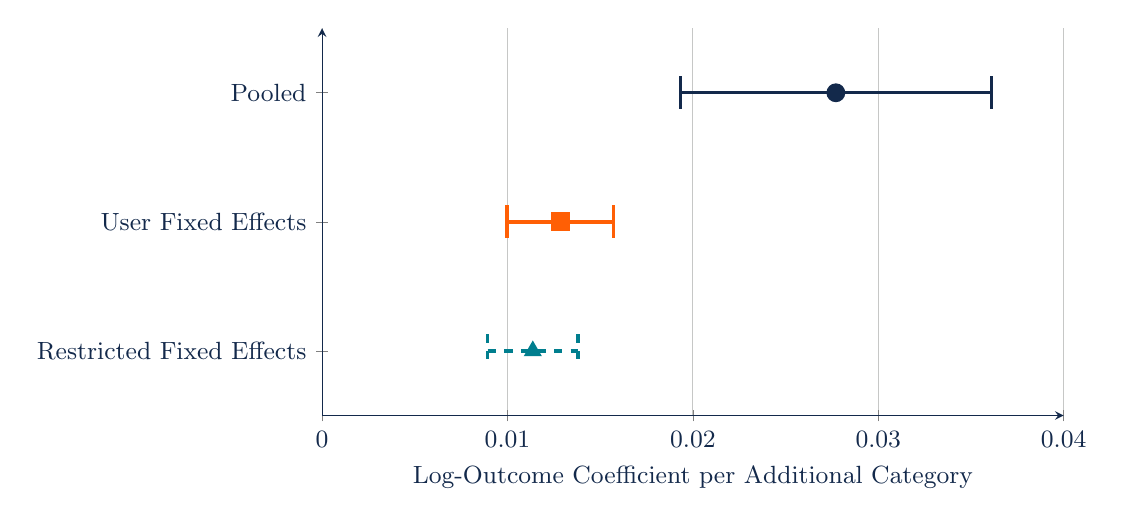
\begin{tikzpicture}
\begin{axis}[xlabel={Log-Outcome Coefficient per Additional Category},xmin=0,xmax=.04,scaled x ticks=false,xtick={0,.01,.02,.03,.04},xticklabel style={/pgf/number format/fixed,/pgf/number format/precision=2},ymin=.5,ymax=3.5,ytick={1,2,3},yticklabels={Restricted Fixed Effects,User Fixed Effects,Pooled},width=11cm,xmajorgrids=true]
\addplot[IlliniBlue,very thick,mark=|,mark size=6pt] coordinates {(.0193357,3)(.0360878,3)};
\addplot[IlliniOrange,very thick,mark=|,mark size=6pt] coordinates {(.0099734,2)(.0157151,2)};
\addplot[Patina,very thick,dashed,mark=|,mark size=6pt] coordinates {(.0089318,1)(.0137982,1)};
\addplot[only marks,IlliniBlue,mark=*,mark size=3pt] coordinates {(.0277117,3)};
\addplot[only marks,IlliniOrange,mark=square*,mark size=3pt] coordinates {(.0128443,2)};
\addplot[only marks,Patina,mark=triangle*,mark size=3pt] coordinates {(.011365,1)};
\end{axis}
\end{tikzpicture}

\end{adjustbox}
\endgroup
\par\medskip
{\small mHealth estimates retain the stated outcome timing and sample restrictions.\par}
\note{A robustness comparison should report which rows change and whether the estimand remains comparable. The range restriction is an imposed screen, not proof that excluded records are incorrect.

M3, Section 3.10, Marketing Analytics Lecture Notes. \url{../06_Lecture_Notes/modules/M03_Regression.md}}
\end{frame}
\begin{frame}[fragile]{A Hand-Checkable Regression}
\usebeamercolor[fg]{normal text}
\noindent Synthetic sales follow a linear relationship.
\begin{lstlisting}
x = [1, 2, 3, 4]
y = [3, 5, 7, 9]
mx, my = sum(x) / 4, sum(y) / 4
b = sum((a-mx)*(v-my) for a,v in zip(x,y))
b /= sum((a-mx)**2 for a in x)
a = my - b * mx
assert (a, b) == (1.0, 2.0)
\end{lstlisting}
{\small The intercept is 1 and the slope is 2 sales units per unit of x.\par}
\note{This example checks the covariance-over-variance calculation. Perfect fit is imposed by construction and is not an empirical finding about marketing behavior.

M3, Section 3.1, Marketing Analytics Lecture Notes. \url{../06_Lecture_Notes/modules/M03_Regression.md}}
\end{frame}
\begin{frame}{Coding Exercise: Regression Checks}
\usebeamercolor[fg]{normal text}
\vfill
\begin{slidebullets}
\item Generate a model after defining the outcome and information set.
\item Verify the coefficient units and one fitted value manually.
\item Compare pooled and customer-effect specifications.
\item Inspect residuals, outliers, and sample changes.
\end{slidebullets}
\vfill
\note{Run the small OLS case in ../03\_Data\_and\_Code/Lecture\_Examples/session\_examples.py S04. The mHealth m03.py program supplies the full real-data calculation, including exact-date pairing and clustered inference.

M3, Section 3.8, Marketing Analytics Lecture Notes. \url{../06_Lecture_Notes/modules/M03_Regression.md}}
\end{frame}
\begin{frame}{Prices Respond to Demand}
\usebeamercolor[fg]{normal text}
\vfill
\begin{slidebullets}
\item Managers can raise prices when demand is unusually strong.
\item An observed price-sales regression can mix demand and pricing choices.
\item An instrument needs relevance and a defensible exclusion restriction.
\end{slidebullets}
\vfill
\note{The course price simulation sets the true elasticity and the source of price endogeneity explicitly. A cost shifter is useful as an instrument only when its other paths to demand can be ruled out under the maintained setting.

M3, Section 3.12, Marketing Analytics Lecture Notes. \url{../06_Lecture_Notes/modules/M03_Regression.md}}
\end{frame}
\begin{frame}{Evidence for an Advertised Claim}
\usebeamercolor[fg]{normal text}
\vfill
\begin{slidebullets}
\item A claim that a product cuts costs needs a suitable comparison.
\item An association can reflect selection and omitted demand.
\item The evidence should support the express and implied claim before publication.
\end{slidebullets}
\vfill
\note{The FTC advertising-substantiation policy requires a reasonable basis for objective claims before dissemination. The necessary support depends on the claim and consequences. This does not turn every regression into an advertising substantiation study.

FTC Policy Statement Regarding Advertising Substantiation. \url{https://www.ftc.gov/legal-library/browse/ftc-policy-statement-regarding-advertising-substantiation}}
\end{frame}
\begin{frame}{Regression Discussion}
\usebeamercolor[fg]{normal text}
\vfill
\begin{slidebullets}
\item Which comparison supports the coefficient?
\item What variable could reverse its interpretation?
\item Would the recommended action change across the reported interval?
\end{slidebullets}
\vfill
\note{A useful interpretation identifies the sample, units, conditioning, and causal scope before a recommendation. The source of variation matters as much as the regression command.

M3, Section 3.8, Marketing Analytics Lecture Notes. \url{../06_Lecture_Notes/modules/M03_Regression.md}}
\end{frame}
\end{document}
